\documentclass{article}

\usepackage[preprint]{neurips_2025}
\usepackage[utf8]{inputenc}
\usepackage[T1]{fontenc}
\usepackage{hyperref}
\usepackage{url}
\usepackage{booktabs}
\usepackage{amsfonts}
\usepackage{amsmath}
\usepackage{nicefrac}
\usepackage{microtype}
\usepackage{xcolor}
\usepackage{graphicx}

\graphicspath{{../docs/figures/}}

\title{LiveTS: A Leakage-Proof, Continuously-Refreshed Benchmark for Zero-Shot Time Series Forecasting}

\author{%
  Anonymous Authors\\
  (LiveTS working draft; author list to be finalized)\\
}

\begin{document}

\maketitle

\begin{abstract}
Time series foundation models (TSFMs) are now routinely evaluated in the ``zero-shot'' regime on benchmarks that predate their pretraining corpora. This creates two failure modes that no amount of statistical care can repair post hoc: (i) \emph{pretraining contamination} --- the test data may literally be in the training set --- and (ii) \emph{community overfitting} --- static test sets are reused across thousands of experiments, turning reported gains into selection effects. We introduce \textbf{LiveTS}, a benchmark that makes both failure modes physically impossible rather than statistically unlikely. LiveTS continuously collects time series from six public real-time domains (energy, weather, air quality, traffic, crypto/FX, and web traffic) with point-in-time snapshot semantics, registers a conservative public release date for every model, and scores a model only on forecast windows whose evaluation cutoff falls \emph{after} that release date (future-only / as-of evaluation). We pre-registered the full protocol --- leakage boundaries, metrics (MASE/CRPS/WQL), geometric-mean aggregation with bootstrap confidence intervals, and Diebold--Mariano tests with Holm correction --- before running the main experiments. Using historical simulation over 205 daily series and three rolling cutoffs (50{,}284 forecast windows), we report the first \emph{clean} scores for six open TSFMs against statistical baselines and supervised baselines retrained strictly before each cutoff. We find no universal winner: TSFMs deliver consistent gains on seasonal domains but fail to beat a seasonal-naive baseline on financial series, and rankings shift across cutoffs --- evidence that single-number leaderboards on static benchmarks overstate what zero-shot forecasting has achieved. LiveTS ships with an open collection pipeline, audit-ready snapshot hashes, and a rolling leaderboard that refreshes monthly, so that the benchmark cannot be overfit faster than reality produces new ground truth.
\end{abstract}

\section{Introduction}

Benchmark evaluation in time series forecasting is facing a quiet crisis. The field's standard test sets --- ETT, Electricity, Traffic, Weather, the Monash archive \citep{godahewa2021monash} --- were assembled years before the current generation of time series foundation models (TSFMs) was trained \citep{ansari2024chronos,das2024timesfm,woo2024moirai,shi2025timemoe}. Modern TSFMs are pretrained on web-scale corpora of public time series; the very datasets used to certify their ``zero-shot'' ability are, at least in part, plausibly inside their training distribution, and in the worst case inside their training set verbatim \citep{meyer2025leakage}. Reported zero-shot numbers are therefore upper bounds of unknown looseness.

A second, older problem compounds the first. Static test sets are evaluated millions of times by a community that collectively tunes architectures, hyperparameters, and random seeds against them. Even with honest individual practice, the community-level process is adaptive data reuse, and the resulting benchmark gains need not transfer.

Both problems share a root cause: \emph{the test data existed before the models did.} We argue the fix must be structural, not statistical. \textbf{LiveTS} evaluates each model only on data generated after the model's weights were publicly released. Contamination and test-set overfitting are then impossible by construction --- a model cannot have been pretrained on data that did not exist, and the community cannot have tuned against ground truth that had not yet been produced.

Our contributions:
\begin{enumerate}
  \item \textbf{A leakage-proof evaluation design} (\S\ref{sec:design}): future-only / as-of evaluation with registered model release dates, rolling cutoffs, point-in-time (PIT) collection semantics, and hashed raw snapshots for audit.
  \item \textbf{A pre-registered protocol} (\S\ref{sec:protocol}, full text in Appendix~A): metrics, aggregation, uncertainty quantification, significance testing, and an amendment policy, frozen before the main experiments.
  \item \textbf{First clean scores} (\S\ref{sec:experiments}): a historical-simulation study over 205 daily series from six domains, three rolling cutoffs, six open TSFMs, statistical baselines (seasonal naive, AutoETS), and supervised baselines (DLinear, PatchTST, iTransformer) retrained strictly before each cutoff --- 50{,}284 forecast windows with full JSONL provenance.
  \item \textbf{A living benchmark} (\S\ref{sec:live}): an open-source collection pipeline running daily across redundant free sources, and a monthly-refresh leaderboard whose ground truth is produced by reality after submissions close.
\end{enumerate}

\section{Related Work}

\paragraph{Static TSFM benchmarks.} GIFT-Eval \citep{aksu2024gifteval} and fev-bench \citep{shchur2025fev} aggregate large collections of public datasets and standardize protocol details, but both are static: their test sets predate the models under evaluation, so pretraining overlap must be handled by best-effort de-duplication, which cannot rule out paraphrased or derived copies \citep{meyer2025leakage}. The Monash archive \citep{godahewa2021monash} is the canonical pre-TSFM benchmark and is now saturated. LiveTS is complementary: it trades corpus breadth for a guarantee no static benchmark can offer.

\paragraph{Live evaluation in other fields.} The M6 competition \citep{makridakis2025m6} ran a genuine live forecasting evaluation but was a one-off event in a single (financial) domain. LiveBench \citep{white2025livebench} and dynamic LLM leaderboards apply the same future-only insight to language models. LiveTS brings this paradigm to multi-domain time series with a reproducible open pipeline.

\paragraph{Evaluation methodology.} A line of work documents protocol inconsistencies (look-back lengths, normalization, per-dataset tuning) that make cross-paper comparisons unreliable \citep{meyer2025leakage}. LiveTS fixes a single pre-registered protocol and forbids per-dataset tuning; its methodological contribution is the combination of PIT data semantics with registered release dates.

\paragraph{Contamination auditing.} Membership-inference and overlap-detection methods estimate contamination post hoc. LiveTS gives the complementary counterfactual: the gap between a model's score on old benchmarks and its clean LiveTS score is an upper bound on what contamination plus community overfitting bought (we develop this analysis jointly with a companion contamination-audit project).

\section{LiveTS Design}\label{sec:design}

\subsection{Data layer}

Six domains, chosen for public availability, daily-or-finer update frequency, key-free access, and at least two redundant sources each: electric grid load/price (NESO UK, SMARD DE), weather station aggregates (Open-Meteo), PM2.5 air quality (Open-Meteo AQ), public transit ridership (NYC MTA/Socrata), crypto and FX rates (Coinbase, ECB/Frankfurter), and Wikipedia pageviews (Wikimedia). A configurable collector runs daily via cron on two geographically separate hosts, stores the raw API response verbatim, tags every record with \texttt{collected\_at} (PIT semantics), and archives snapshots to object storage with a SHA-256 manifest so that any later revision of source data is detectable. The evaluation set currently spans \textbf{205 daily series} (weather 80, web traffic 58, crypto/FX 34, air quality 20, traffic 7, energy 6); the series list is configuration, not code, and grows without changing the protocol.

\subsection{Leakage boundary: release dates and future-only scoring}

Every evaluated model registers a \textbf{release date}: the earliest publicly verifiable timestamp of its weights (we use the Hugging Face repository creation date; when in doubt, the earlier date is used --- conservative in the direction of \emph{fewer} clean windows). Given rolling cutoffs $c_1 < c_2 < \dots$, a model's clean score aggregates only forecast windows with cutoff $>$ release date. Inputs at each forecast origin are strictly pre-origin observations; targets are the subsequent horizon. In live rounds the target values physically do not exist at submission time; the historical-simulation study in \S\ref{sec:experiments} replays the same rule against archived history, which is exact provided the model's weights were frozen at its release date.

\subsection{Pre-registered protocol}\label{sec:protocol}

Frozen 2026-08-09 (summary; full text Appendix~A). Three cutoffs (2025-01-01, 2025-07-01, 2026-01-01); four forecast origins per cutoff drawn from the 180 days following it; horizon 14 at daily frequency; look-back = each model's maximum context up to 2048 points, identical across domains; no per-dataset tuning of any kind. Metrics: MASE \citep{hyndman2006mase} (seasonal in-sample naive scale; period 7 for seasonal domains, 1 for financial), CRPS approximated from nine deciles \citep{gneiting2007crps}, and weighted quantile loss (WQL). Aggregation: arithmetic mean over origins $\times$ seeds within a series, then geometric mean across series; 95\% CIs from a cross-series bootstrap ($B{=}1000$). Sampling-based models run seeds $\{0,1,2\}$; deterministic models are flagged. Significance: paired bootstrap and Diebold--Mariano \citep{diebold1995dm} with the Harvey--Leybourne--Newbold small-sample correction \citep{harvey1997hln} on shared windows, Holm-corrected \citep{holm1979} at $\alpha{=}0.05$. Point-only models receive no probabilistic score (we do not impute quantiles from point forecasts). Supervised baselines are retrained from scratch on strictly pre-cutoff data for every cutoff, making every cutoff clean for them by construction.

\subsection{Service layer}

Snapshots and manifests live in object storage (Cloudflare R2); a monthly evaluation round opens after each cutoff, accepts one submission per model per round, and publishes scores when the target window has fully materialized. New models must register a release date before their first round; protocol changes are timestamped amendments that never retroactively alter published scores.

\section{Historical-Simulation Experiments}\label{sec:experiments}

\subsection{Setup}

205 series $\times$ 3 cutoffs $\times$ 4 origins $\times$ horizon 14 ($\approx$2{,}460 windows per deterministic model; $\times$3 seeds for sampling models and supervised baselines). Models: seasonal naive; AutoETS; DLinear \citep{zeng2023dlinear}, PatchTST \citep{nie2023patchtst}, iTransformer \citep{liu2024itransformer} (global models, retrained pre-cutoff, multi-quantile loss, 3 seeds); Chronos-Bolt-small/base and Chronos-T5-small \citep{ansari2024chronos}; Time-MoE-50M \citep{shi2025timemoe} (point-only); Moirai-1.1-R-small \citep{woo2024moirai}; TimesFM-2.5-200M \citep{das2024timesfm}. All zero-shot inference used a single configuration per model across all domains. Every result row carries the git commit, environment versions, and run timestamp (JSONL, open).

\subsection{Main results}

\begin{table}[t]
  \caption{Clean scores on LiveTS (historical simulation, 205 series, future-only cutoffs). Geometric mean across series of per-series mean MASE/WQL; 95\% cross-series bootstrap CI ($B{=}1000$). $^{\dagger}$fewer than three clean cutoffs due to release-date gating --- compare on overlapping cutoffs only. Supervised baselines (release ``per-cutoff'') are retrained strictly pre-cutoff, so every cutoff is clean for them.}
  \label{tab:main}
  \centering
  \small
  \begin{tabular}{lccccc}
\toprule
Model & Release & geo-MASE [95\% CI] & geo-WQL & Series & Windows \\
\midrule
timesfm-2.5-200m$^{\dagger}$ & 2025-09-02 & 0.789 [0.711, 0.873] & 0.120 & 205 & 820 \\
chronos-bolt-small & 2024-11-25 & 0.893 [0.817, 0.976] & 0.127 & 207 & 2484 \\
chronos-bolt-base & 2024-11-25 & 0.895 [0.826, 0.980] & 0.127 & 207 & 2484 \\
chronos-t5-small & 2024-02-21 & 0.956 [0.877, 1.048] & 0.132 & 205 & 7380 \\
moirai-1.1-r-small & 2024-06-14 & 0.965 [0.880, 1.051] & 0.140 & 205 & 7380 \\
time-moe-50m & 2024-09-21 & 1.004 [0.923, 1.111] & --- & 205 & 2460 \\
patchtst & per-cutoff & 1.099 [1.019, 1.185] & 0.179 & 207 & 7452 \\
autoets & --- & 1.133 [1.050, 1.223] & 0.212 & 205 & 2460 \\
seasonal\_naive & --- & 1.181 [1.092, 1.268] & 0.200 & 205 & 2460 \\
dlinear & per-cutoff & 1.597 [1.428, 1.788] & 0.334 & 207 & 7452 \\
itransformer & per-cutoff & 4.220 [3.860, 4.627] & 0.933 & 207 & 7452 \\
\bottomrule
\end{tabular}

\end{table}

\begin{table}[t]
  \caption{Per-domain geo-MASE. No model wins everywhere; on crypto/FX no model beats seasonal naive except TimesFM-2.5 on its single clean cutoff.}
  \label{tab:domain}
  \centering
  \scriptsize
  \begin{tabular}{lcccccc}
\toprule
Model & air\_quality & crypto\_fx & energy & traffic & weather & web\_traffic \\
\midrule
timesfm-2.5-200m & 0.75 & 2.16 & 0.93 & 0.75 & 0.68 & 0.54 \\
chronos-bolt-small & 0.79 & 2.66 & 0.90 & 1.24 & 0.70 & 0.67 \\
chronos-bolt-base & 0.79 & 2.75 & 0.89 & 1.19 & 0.70 & 0.67 \\
chronos-t5-small & 0.83 & 2.98 & 0.97 & 1.46 & 0.75 & 0.68 \\
moirai-1.1-r-small & 0.83 & 2.75 & 1.03 & 1.61 & 0.76 & 0.72 \\
time-moe-50m & 0.81 & 3.60 & 0.89 & 1.04 & 0.80 & 0.71 \\
patchtst & 0.85 & 2.98 & 1.02 & 1.28 & 0.95 & 0.82 \\
autoets & 1.17 & 2.57 & 1.25 & 1.39 & 0.93 & 0.88 \\
seasonal\_naive & 1.04 & 2.57 & 1.30 & 1.71 & 1.05 & 0.87 \\
dlinear & 1.02 & 8.01 & 1.17 & 1.46 & 1.25 & 1.08 \\
itransformer & 2.74 & 13.61 & 3.16 & 9.00 & 3.46 & 3.08 \\
\bottomrule
\end{tabular}

\end{table}

\begin{figure}[t]
  \centering
  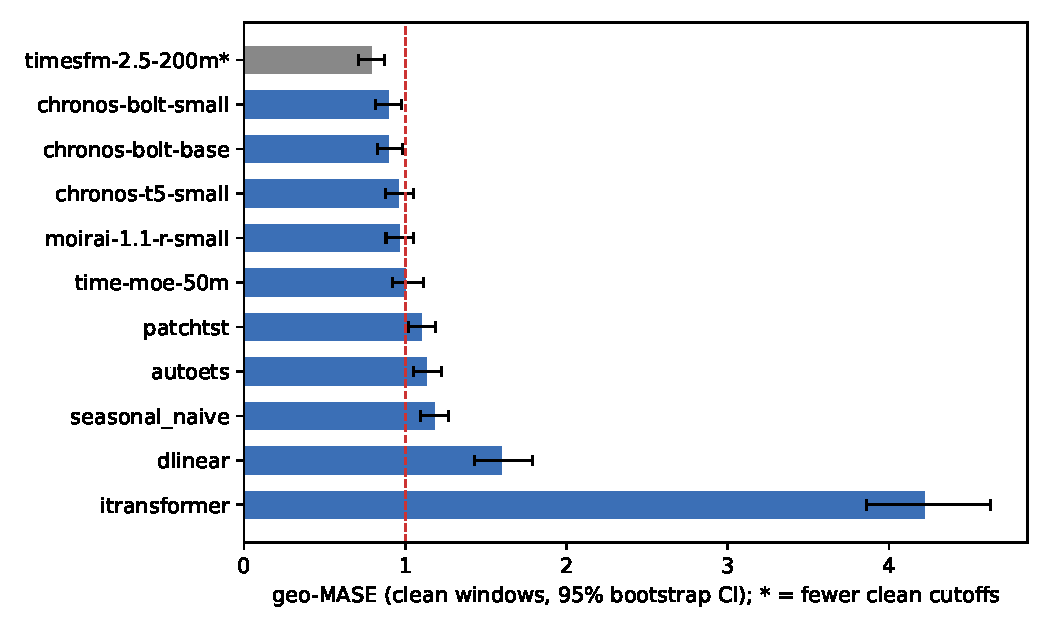
\includegraphics[width=0.85\linewidth]{fig1_main_geomase.pdf}
  \caption{Clean geo-MASE with 95\% bootstrap CIs. Grey bar: model with fewer clean cutoffs (release-date gating); dashed line: seasonal-naive parity.}
  \label{fig:main}
\end{figure}

\begin{figure}[t]
  \centering
  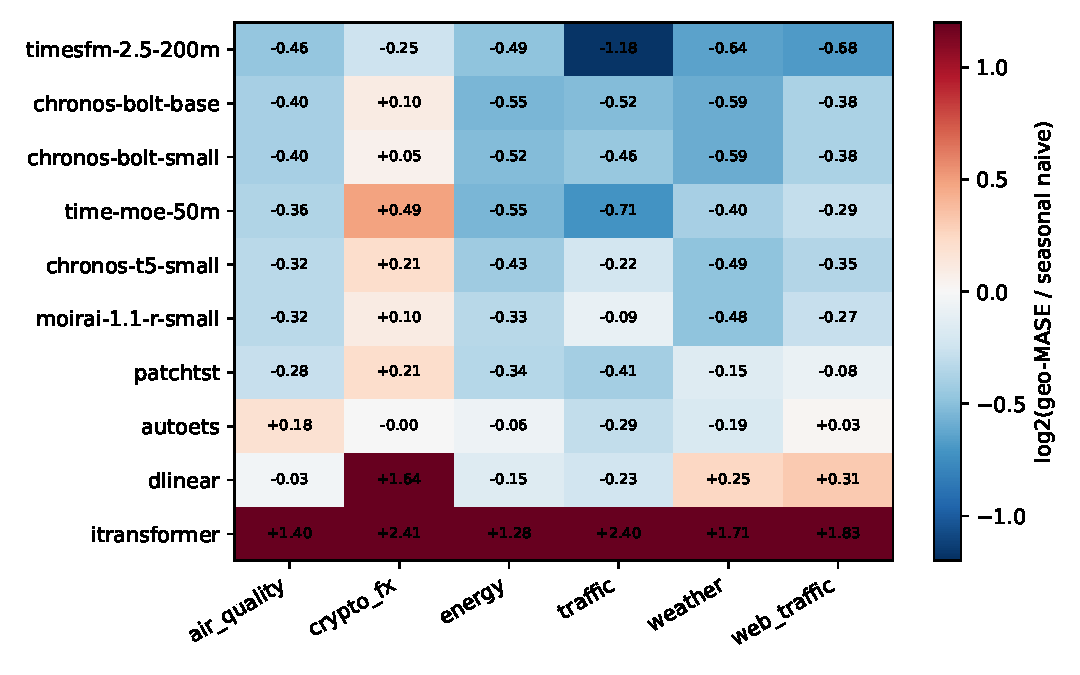
\includegraphics[width=0.9\linewidth]{fig2_domain_heatmap.pdf}
  \caption{Per-domain geo-MASE relative to seasonal naive ($\log_2$ ratio; blue = better than naive). TSFMs win on seasonal domains and lose on crypto/FX.}
  \label{fig:heatmap}
\end{figure}

Table~\ref{tab:main} and Figure~\ref{fig:main} report the main results; Table~\ref{tab:domain} and Figure~\ref{fig:heatmap} break them down by domain. Three observations:

\begin{enumerate}
  \item \textbf{Release-date gating matters.} TimesFM-2.5's clean score covers only the cutoff after its 2025-09 release; comparing it to models with three clean cutoffs on the pooled table would be flattering nonsense. LiveTS makes this visible instead of averaging it away. On shared windows, TimesFM-2.5 is significantly better than every other model after Holm correction except Chronos-Bolt-base, where the difference does not survive correction (Appendix~C).
  \item \textbf{No universal winner.} On financial series (crypto/FX), no TSFM with three clean cutoffs beats seasonal naive on MASE (TimesFM-2.5 does on its single clean cutoff) --- consistent with near-martingale dynamics --- while on seasonal domains (weather, air quality, traffic, web) TSFMs deliver 10--40\% MASE improvements (Figure~\ref{fig:heatmap}).
  \item \textbf{Significance survives correction only for the largest gaps.} After Holm correction, Chronos-Bolt (small/base) and Moirai are significantly better than seasonal naive, but Chronos-T5-small and Time-MoE are not; PatchTST is statistically indistinguishable from seasonal naive and AutoETS on shared windows; several pairwise TSFM comparisons that look decisive as point estimates are not significant (Appendix~C).
\end{enumerate}

Supervised baselines were retrained pre-cutoff with a fixed generic configuration (multi-quantile loss, input size 96, 1000 steps, no per-dataset tuning). PatchTST is competitive with weaker TSFMs; DLinear and iTransformer underperform under this no-tuning regime. iTransformer runs in univariate mode ($n_{\text{series}}{=}1$), a conservative configuration at odds with its multivariate design; we report it as a lower bound and note this as a limitation rather than tuning it post hoc.

\subsection{Robustness}

\begin{figure}[t]
  \centering
  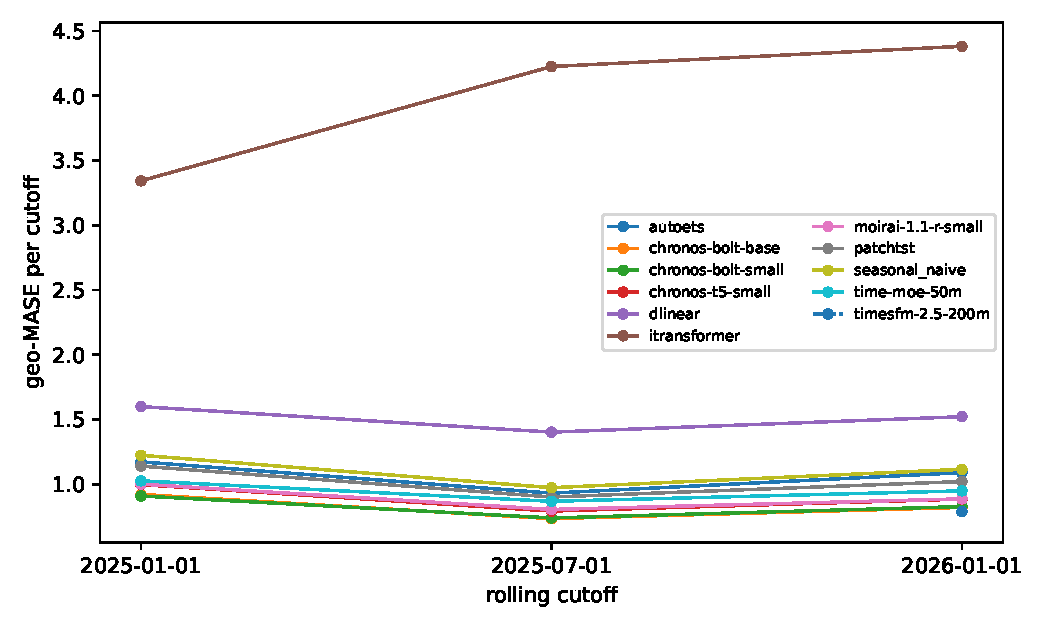
\includegraphics[width=0.8\linewidth]{fig3_cutoff_shift.pdf}
  \caption{Per-cutoff geo-MASE. Mid-table rankings shift across cutoffs; a single static split would misrank models.}
  \label{fig:cutoff}
\end{figure}

Figure~\ref{fig:cutoff} shows per-cutoff scores: mid-table rankings (Chronos-T5 vs.\ Moirai vs.\ Time-MoE vs.\ PatchTST) reorder across cutoffs, while the top (Chronos-Bolt) and bottom are stable. Seed variance for sampling models is small relative to cross-series dispersion. This is quantitative evidence that a single static split materially misranks models --- and an argument for rolling evaluation as the default.

\subsection{Clean scores vs.\ post-hoc contamination signals}\label{sec:contamination}

A companion contamination audit\footnote{\url{https://github.com/wookat/tsfm-contamination-audit}; 8 TSFMs $\times$ 14 datasets, member vs.\ non-member skill probes with permutation tests and Holm correction.} probes the same model families post hoc: for each TSFM it contrasts forecasting skill on \emph{member} datasets (documented in the model's pretraining corpus) against \emph{non-member} datasets. Table~\ref{tab:contamination} places its skill-probe results next to our clean LiveTS scores.

\begin{table}[t]
  \caption{LiveTS clean skill vs.\ post-hoc audit signals. skill$_{\text{live}}$ = geo-MASE(model)/geo-MASE(seasonal naive) on shared clean windows (lower is better). Audit columns: mean skill on member vs.\ non-member datasets and Holm-corrected permutation $p$; a positive member$-$non-member gap is directionally consistent with contamination-inflated legacy scores. $^{a}$audited checkpoint differs from the one we evaluate (Moirai-1.0-R-small; TimesFM-2.0-500M) --- directional reference only.}
  \label{tab:contamination}
  \centering
  \small
  \begin{tabular}{lcccc}
    \toprule
    Model & skill$_{\text{live}}$ & Audit member & Audit non-member & Holm $p$ \\
    \midrule
    Chronos-Bolt-small & 0.754 & 0.297 & $-0.673$ & 0.86 \\
    Chronos-Bolt-base & 0.756 & 0.323 & $-1.088$ & 0.62 \\
    Chronos-T5-small & 0.809 & 0.253 & $-0.108$ & 1.00 \\
    Time-MoE-50M & 0.850 & $-0.382$ & 0.173 & 1.00 \\
    Moirai-1.1-R-small & 0.817 & $-0.216^{a}$ & $0.026^{a}$ & 1.00 \\
    TimesFM-2.5-200M & 0.707 & $0.417^{a}$ & $-0.134^{a}$ & 0.24 \\
    \bottomrule
  \end{tabular}
\end{table}

The audit finds member-dataset skill consistently higher for the Chronos family and TimesFM (Cliff's $\delta$ 0.47--0.85), directionally consistent with contamination-inflated legacy scores, but no effect survives Holm correction at the audit's sample size --- post-hoc detection is statistically underpowered even when the direction is consistent. This is precisely the argument for LiveTS: rather than trying to detect contamination after the fact, future-only evaluation makes it impossible. The two approaches are complementary; LiveTS clean scores are currently the only scores for these models that the contamination question cannot touch.

\section{The Live Benchmark}\label{sec:live}

Round-0 opens with the protocol frozen in Appendix~A. Monthly cadence: cutoff on the 1st, submissions within 7 days (forecasts only --- no post-cutoff data access), scoring after the 14-day target window completes, publication with full JSONL provenance. Anti-gaming: one submission per model per round; release-date registration precedes first participation; raw snapshot hashes published for third-party audit; the aggregation code is deterministic and open.

\section{Limitations and Ethics}

Univariate daily-frequency focus (intraday and multivariate tracks are future work); free-tier sources can rate-limit or discontinue (mitigated by $\geq$2 sources per domain, but a domain could still degrade); public infrastructure data skews toward well-instrumented regions; release dates rely on public timestamps and may be later than private availability (our conservative rule errs toward fewer clean windows, not more). Supervised baselines use one generic configuration --- their scores are lower bounds, not the best achievable. The benchmark evaluates forecast quality only; downstream decision costs are out of scope.

\bibliographystyle{plainnat}
\bibliography{references}

\appendix

\section{Pre-registered protocol v1.0 + amendment A1}
The full pre-registration (frozen 2026-08-09) is distributed with the benchmark repository (\texttt{docs/protocol-prereg.md}); amendment A1 (series expansion 25$\to$205 and supervised baselines) was registered before the expanded runs and does not alter previously published results.

\section{Data sources and series list}
See \texttt{docs/data-sources.md} and the generated series inventory in the repository. Every series has $\geq$800 daily points ($\geq$700 for FX, trading-day calendar).

\section{Full significance matrices}
The full pairwise matrix (56 pairs, paired bootstrap $B{=}10{,}000$ and DM--HLN, Holm-corrected) is generated by \texttt{scripts/significance.py} and distributed as \texttt{docs/significance.md}.

\section{Reproduction}
One command per table; JSONL schema; environment lockfiles; commit hashes. See \texttt{REPRODUCIBILITY.md} in the repository.

\end{document}
